\section{Safety-Constrained CoC와 평가 방법}
\label{sec:method}

본 장의 목적은 모델이 실행 가드를 실제로 읽고 궤적 선택에 사용하는지 확인하는 방법을 설명하는 것이다. 이를 분명하게 측정하기 위해 모델이 새로운 궤적을 직접 만들게 하지 않고, 미리 만든 여러 후보 중 하나를 고르게 한다. 모델이 직접 궤적을 만들면 궤적 생성 능력과 가드 이해 능력이 결과에 함께 섞인다. 후보 선택 문제로 범위를 좁히면, 같은 후보를 놓고 가드가 바뀔 때 모델의 선택도 바뀌는지를 직접 확인할 수 있다.

\revtwo{3장의 최적화 정의를 실제 평가 절차로 옮기기 위해 이 장은 세 질문에 순서대로 답한다. 모델에 무엇을 입력하는가, 가드 사용 여부를 어떤 대조군과 쌍대 계약으로 분리하는가, 그리고 선택 결과를 모델과 독립된 규칙으로 어떻게 판정하는가이다. 따라서 제안 방법의 출력은 연속 제어 명령이 아니라 후보 식별자이며, 검증기는 그 후보의 저장 측정값을 계약 경계와 비교한다.}

\subsection{제안 방법의 전체 흐름}

그림~\ref{fig:pipeline}의 과정은 세 단계로 이루어진다. 첫째, 모델에 장면 이미지, 기본 CoC, 실행 가드와 궤적 후보를 준다. 기본 CoC는 "보행자에게 양보한 뒤 진행한다"처럼 달성할 행동을 말한다. 실행 가드는 "정지선을 넘지 않는다" 또는 "차량이나 보행자의 이동 경로가 겹치는 구역이 1.5초 동안 비어 있을 때만 출발한다"처럼 그 행동을 언제, 어느 범위에서 허용할지를 정한다. 각 후보에는 정지 위치, 속도, 감속도, 가가속도(가속도가 변하는 정도), 차량 간격과 진입 시점이 함께 적혀 있다.

둘째, 모델은 이미지와 문장을 읽고 후보 하나를 선택한다. 셋째, 모델 외부의 결정적 검증기(verifier)가 선택된 후보의 수치를 다시 계산한다. 예를 들어 정지선을 넘었는지, 최소 간격을 지켰는지, 필요한 시간만큼 기다렸는지를 확인한다. 따라서 모델이 스스로 "안전하다"고 답한 것만으로 정답으로 인정하지 않는다. 모델의 선택과 검증기의 계산 결과가 모두 맞아야 가드를 지킨 선택으로 판정한다. 다만 후보 수치, 정답 생성 규칙과 검증 규칙은 같은 합성 과제 정의에서 만들어졌으므로, 이 검증기는 모델과는 분리되어 있지만 계약 자체의 타당성을 확인하는 외부 안전 정답은 아니다.

\begin{figure*}[!t]
\centering
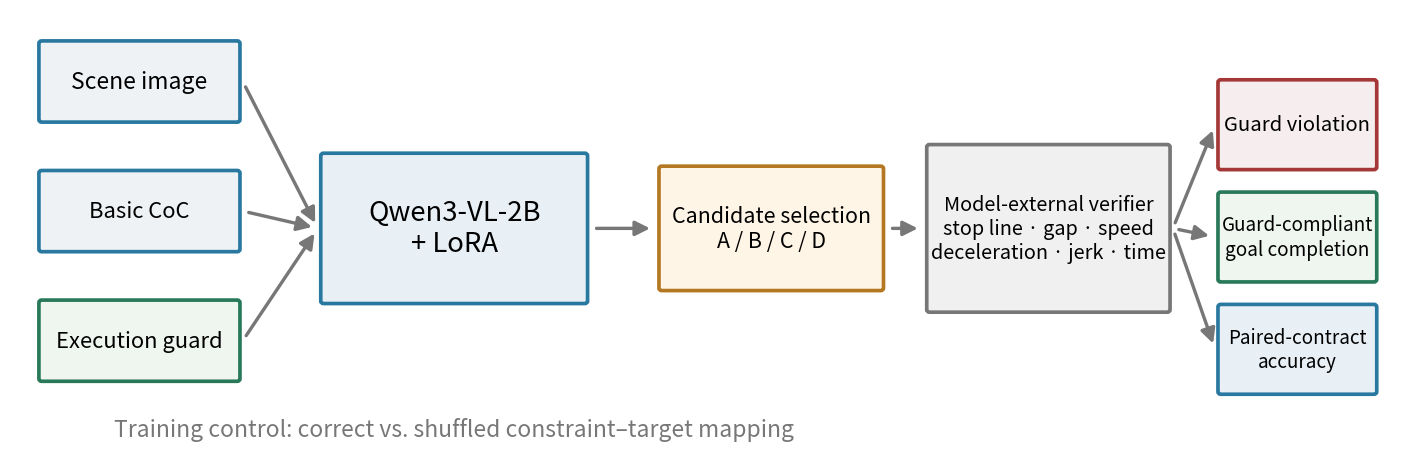
\includegraphics[width=0.98\textwidth]{../latex-kiee-review-2022/figures/fig02_pipeline.png}
\bifigcaption{제안 평가의 흐름. 왼쪽의 장면ㆍ기본 CoCㆍ실행 가드를 모델에 입력하면 모델이 가운데의 후보 A--D 중 하나를 선택한다. 오른쪽의 규칙 기반 검증기는 선택된 후보의 정지 위치, 간격, 속도 및 시간을 가드의 기준값과 비교하여 가드 위반률, 가드 준수 목표 완료율 및 계약 쌍 정확도를 계산한다. 검증기는 모델의 자기평가가 아니라 후보 수치에 결정 규칙을 적용한다.}{Evaluation pipeline from scene, basic CoC, and execution guard through candidate selection to model-external deterministic metric computation.}
\label{fig:pipeline}
\end{figure*}

\subsection{CoC와 실행 가드의 입력 방식}

본 연구는 기본 CoC에 실행 가드를 결합한 형식을 제안한다. 예를 들어 기본 CoC가 "횡단보도 앞 보행자에게 양보한 뒤, 허용되면 진행한다"라면 다음 조건을 덧붙일 수 있다.

\begin{quote}\small
정지선을 넘지 않는다. 최대 감속도는 $3.8\,\mathrm{m/s^2}$, 최대 가가속도는 $5.0\,\mathrm{m/s^3}$를 넘지 않는다. 상충 구역이 정해진 시간 동안 비어 있을 때만 출발한다.
\end{quote}

이 실행 가드를 기본 CoC 뒤에 이어서 한 문장 묶음으로 제시한 방식을 \textbf{제약 통합 CoC}라 한다. 이것이 본 논문의 Safety-Constrained CoC를 실험에 구현한 제안 조건이다. 모델은 이 입력에서 "무엇을 해야 하는가"와 "그 행동을 언제 허용하는가"를 함께 읽는다. 다만 성능이 좋아지더라도 그 이유가 가드의 의미를 배웠기 때문인지, 단순히 문장이 더 길어졌기 때문인지 구분해야 한다. 이를 위해 표~\ref{tab:representations}의 다섯 조건을 비교한다. 표와 그림 내부는 영어로 통일하여 각각 \textit{Basic CoC (no constraint)}, \textit{Constraint-integrated CoC (proposed)}, \textit{Separate natural-language constraint}, \textit{Shuffled constraint--target mapping}, \textit{Logical-form constraint}로 표시한다.

\begin{table*}[!t]
\centering
\bitablecaption{실험 조건의 공통 이름과 차이. `제약 통합 CoC'는 제안 조건이며, `제약--정답 대응 교란'은 제약 문장의 추가 효과와 올바른 의미 대응의 효과를 구분하기 위한 음성 통제군이다.}{Common names and differences among input conditions. The shuffled constraint--target condition is a negative control.}
\label{tab:representations}
\footnotesize
\begin{tabularx}{\textwidth}{L{0.19\textwidth}L{0.25\textwidth}Y}
\toprule
Condition & Model input & Purpose \\
\midrule
Basic CoC (no constraint) & Basic CoC describing only the behavioral objective & Information-absent baseline that cannot distinguish the two contracts \\
Constraint-integrated CoC (proposed) & Natural-language execution guard appended directly to the basic CoC & Learn the objective and admissibility conditions in one context \\
Separate natural-language constraint & The same natural-language guard supplied in a separate input field & \revone{Position-only ablation: preserve guard wording, examples, and training budget while changing its placement} \\
Shuffled constraint--target mapping & A constraint is supplied, but training pairs it with another example's target & Test whether correct constraint--action correspondence is necessary \\
Logical-form constraint & The same execution condition written in a fixed logical form & Test whether the current model handles a structured non-natural-language form \\
\bottomrule
\end{tabularx}
\end{table*}

특히 \textbf{제약--정답 대응 교란}은 음성 통제군이지 제안 방법이 아니다. 이 조건에도 동일한 제약 문장 집합이 들어가지만, 학습할 때 다른 예의 제약 문장을 옮겨 제약과 정답 후보의 연결을 깨뜨린다. 평가는 다시 올바른 제약으로 수행한다. 따라서 올바른 대응을 학습한 조건만 높은 성능을 보인다면, 단순히 문장이 길어지거나 제약 관련 단어가 들어간 효과로 설명하기 어렵다.

\revone{시간 과제에서는 두 개의 통제된 대비를 분리한다. 첫째, 제약 통합 CoC와 별도 자연어 제약은 동일한 가드 문장, 장면, 후보, 정답, 384개 학습 예, 3 epoch 및 최적화 설정을 사용한다. 차이는 가드를 기본 CoC 문장 뒤에 이어 붙이는지, 동일 문장을 별도 \texttt{Temporal safety guard} 필드에 두는지뿐이므로 이 비교는 위치ㆍ구획 형식의 효과를 측정하는 position-only ablation이다. 둘째, 별도 자연어 제약과 제약--정답 대응 교란은 입력 위치를 같게 유지하고 학습 시 가드와 정답의 대응만 깨뜨리므로 올바른 의미 대응의 필요성을 측정한다. 이 두 대비는 위치 효과와 대응 효과를 구분하지만, 시간 과제에 통합 위치의 대응 교란 조건이 없으므로 완전한 $2\times2$ 요인 설계는 아니다. 따라서 제약 통합 CoC와 대응 교란의 전체 차이를 의미 학습만의 효과로 해석하지 않는다. 다중 주행 과제에서는 제약 통합 CoC와 대응 교란이 같은 형식이다. \textbf{논리식 제약}도 자연어와 논리식 중 어느 쪽이 본질적으로 우수한지 판정하기 위한 조건이 아니라, 현재 VLM과 학습 방법이 두 표현을 얼마나 잘 처리하는지 확인하기 위한 조건이다.}

\subsection{같은 장면에서 실행 조건만 바꾸는 평가}

한 장면으로 정답이 서로 다른 두 문제를 만든다. 두 문제에는 같은 이미지, 같은 CoC 목표와 같은 궤적 후보를 사용한다. 바꾸는 것은 실행 가드뿐이다. 가드가 달라지면 올바른 후보도 달라지게 구성한다. 따라서 모델이 두 문제를 모두 맞히려면 장면만 보고 같은 답을 반복해서는 안 되고, 가드를 읽은 뒤 선택을 바꾸어야 한다. 이 두 문제의 묶음을 \textbf{쌍대 계약(paired-contract)}이라 한다.

그림~\ref{fig:pair}은 차선 변경 예에서 무엇이 고정되고 무엇이 바뀌는지를 보여준다. 두 계약 모두 현재 차량 간격은 7.2 m이며 후보도 같다. 후보 A는 현재 간격에서 바로 차선을 변경하고, 후보 B는 차선 변경을 중단한 뒤 필요한 간격이 확보되면 다시 시도한다. 최소 간격이 5.5 m인 완화 계약에서는 $7.2 \geq 5.5$이므로 후보 A가 허용되고 진행도가 높은 후보 A를 선택한다. 반면 최소 간격이 9.0 m인 엄격 계약에서는 $7.2 < 9.0$이므로 후보 A가 가드를 위반하고 후보 B를 선택해야 한다.

즉, 완화 계약과 엄격 계약은 장면이 아니라 허용 기준만 다르다. 모델이 두 문제에 같은 후보를 답하면 적어도 하나는 틀린다. "계약 쌍 정확도"는 두 문제를 모두 맞혔을 때만 그 쌍을 정답으로 계산한다. 이 값이 높을수록 모델이 최소 간격의 변화를 읽고 선택에 반영했다고 볼 수 있다.

\begin{figure*}[!t]
\centering
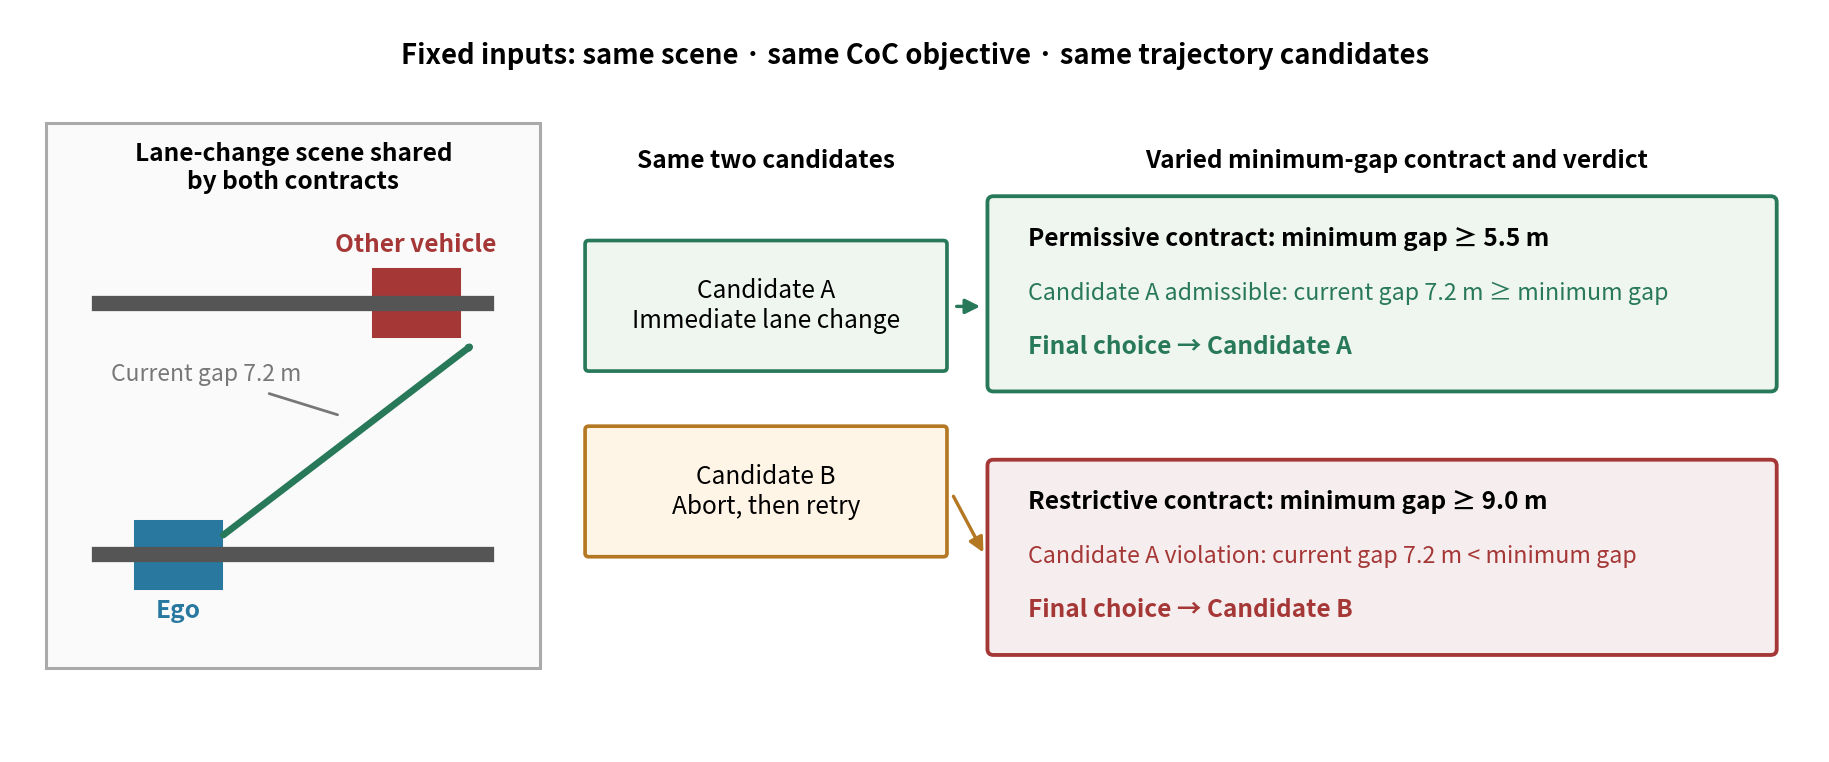
\includegraphics[width=0.98\textwidth]{../latex-kiee-review-2022/figures/fig03_paired_contract.png}
\bifigcaption{쌍대 계약의 차선 변경 예. 장면, CoC 목표, 현재 간격 7.2 m 및 후보 A/B는 고정하고 최소 간격만 5.5 m에서 9.0 m로 바꾼다. 완화 계약에서는 즉시 차선 변경하는 후보 A가 허용되지만, 엄격 계약에서는 같은 후보가 최소 간격을 위반하므로 중단 후 재시도하는 후보 B를 선택한다.}{Paired-contract lane-change example with fixed scene, objective, current gap, and candidates but different minimum-gap contracts.}
\label{fig:pair}
\end{figure*}

시간 과제에서는 행동이 다른 네 후보를 사용한다. 모델은 $A$, $B$, $C$, $D$ 중 하나를 답하지만, 이 문자는 후보를 구별하기 위한 이름일 뿐이다. 예를 들어 $A$가 언제나 조기 진입을 뜻하는 것은 아니다. 표~\ref{tab:candidate-roles}은 후보가 실제로 수행하는 네 가지 행동을 보여준다.

\begin{table*}[!t]
\centering
\bitablecaption{시간 과제 후보를 행동 의미로 해석하는 방법. 행은 후보 문자가 아니라 실제 행동 역할이며, 열은 같은 장면에 적용한 짧은 대기(완화)와 긴 대기(엄격) 계약의 판정이다. 완화 계약은 짧은 대기 후 진입, 엄격 계약은 긴 대기 후 진입을 정답으로 만든다.}{Behavioral roles of temporal candidates under short-wait permissive and long-wait restrictive contracts.}
\label{tab:candidate-roles}
\footnotesize
\begin{tabularx}{\textwidth}{L{0.18\textwidth}L{0.29\textwidth}L{0.20\textwidth}Y}
\toprule
Trajectory role & Behavior & Permissive contract & Restrictive contract \\
\midrule
Early entry & Enter before the conflict zone becomes clear & Guard violation & Guard violation \\
Entry after a short hold & Proceed after a short clear-zone hold & Preferred admissible candidate & Violation: insufficient hold time \\
Entry after a long hold & Proceed after a longer confirmation interval & Admissible but less progress & Preferred goal-completing candidate \\
Remain stopped & Stay stopped until the evaluation ends & Goal incomplete or deadlock & Goal incomplete or deadlock \\
\bottomrule
\end{tabularx}
\end{table*}

한 장면에서는 $A$가 조기 진입이고 $B$가 짧은 대기일 수 있다. 다음 장면에서는 문자와 행동의 대응을 바꾸어 $A$가 긴 대기를 나타내게 할 수 있다. 이렇게 하면 모델이 항상 같은 문자만 고르는 방법으로 정답을 외울 수 없다. 정적 실험은 두 후보 $A/B$를, 시간 및 다중 주행 실험은 네 후보 $A/B/C/D$를 사용한다. 어느 실험에서도 특정 문자가 항상 안전하거나 항상 위험한 행동을 뜻하지 않는다.

\subsection{모델 학습과 정답 후보 생성}

기반 모델은 Qwen3-VL-2B-Instruct이다. 전체 모델을 다시 학습하지 않고 일부 추가 매개변수만 조정하는 LoRA 방식을 사용한다. 모델이 한 번에 받는 학습 자료는 다음 다섯 부분으로 구성된다.

\begin{enumerate}
\item 장면을 나타내는 합성 이미지,
\item 달성해야 할 행동을 설명하는 기본 CoC,
\item 실험 조건에 따른 실행 가드,
\item 각 후보의 행동과 측정값을 적은 설명,
\item 허용되는 후보 중 진행도가 가장 높은 후보를 고르라는 지시.
\end{enumerate}

모델은 후보 문자 하나를 답한다. 정답은 다음 세 단계로 정한다. 먼저 CoC의 행동 목표를 끝내지 못한 후보를 제외한다. 그다음 실행 가드를 위반한 후보를 제외한다. 마지막으로 남은 후보 중에서 가장 원활하게 진행하는 후보를 정답으로 삼는다. 모든 장면에는 목표와 가드를 함께 만족하는 후보가 적어도 하나 있다. 이는 식~\eqref{eq:selection}을 학습 자료 생성에 그대로 적용한 것이다.

예를 들어 가장 빨리 진행하는 후보가 최소 간격을 위반하면 정답이 될 수 없다. 반대로 가드 위반을 피하기 위해 끝까지 정지하는 후보도 행동 목표를 완료하지 못하므로 정답이 아니다. 모델은 "진행"과 "가드 준수"를 동시에 만족하는 후보를 찾아야 한다.

\subsection{모델 외부 궤적 검증과 평가 지표}

모델의 답은 $A$와 같은 후보 문자일 뿐이다. 이 답이 실제로 가드를 지켰는지는 별도 검증기가 계산한다. 검증기는 표~\ref{tab:verifier-fields}의 수치를 후보 데이터에서 읽고 가드의 기준과 직접 비교한다. 예를 들어 최소 간격이 9.0 m라면 선택한 후보의 간격이 9.0 m 이상인지 확인한다.

\begin{table}[t]
\centering
\bitablecaption{모델 외부 검증기의 판정값과 읽는 법. 검증기는 모델의 설명을 믿지 않고 선택된 후보의 저장 수치를 계약 경계와 직접 비교한다.}{Values used by the model-external deterministic verifier, which compares stored candidate measurements directly with contract bounds.}
\label{tab:verifier-fields}
\footnotesize
\begin{tabularx}{\columnwidth}{L{0.34\columnwidth}Y}
\toprule
Checked value & Example decision \\
\midrule
Stop-line-relative position & Crossing is detected when the position exceeds 0 m \\
Maximum speed & Check whether the allowed speed limit is exceeded \\
Maximum deceleration & Check whether the hard-braking limit is exceeded \\
Maximum jerk & Check whether the acceleration-change limit is exceeded \\
Minimum vehicle gap & Check whether the required distance to another vehicle is maintained \\
Intersection entry time & Check the required hold after the conflict zone becomes clear \\
\bottomrule
\end{tabularx}
\end{table}

표~\ref{tab:method-metrics}은 평가에 사용한 지표를 정리한다. 비율의 분모는 별도 표기가 없으면 해당 평가의 전체 예다. 이 가운데 "가드 준수 목표 완료율"은 두 가지를 동시에 만족한 비율이다. 첫째, 선택한 후보가 CoC의 행동 목표를 완료해야 한다. 둘째, 실험에서 제시한 실행 가드를 모두 지켜야 한다. 이 지표는 실제 도로의 모든 위험이 제거되었다는 뜻은 아니다.

\begin{table}[t]
\centering
\bitablecaption{표와 그림에 반복해서 사용하는 지표. 후보 정확도ㆍ가드 준수 목표 완료율ㆍ계약 쌍 정확도는 높을수록 좋고, 가드 위반률ㆍ교착률ㆍ과도한 보수 선택률은 낮을수록 좋다.}{Metrics used throughout the tables and figures, including their preferred directions.}
\label{tab:method-metrics}
\footnotesize
\begin{tabularx}{\columnwidth}{L{0.31\columnwidth}Y}
\toprule
Metric & Meaning \\
\midrule
Candidate accuracy & Fraction selecting the optimal candidate defined by the data-generation rule \\
Guard violation rate & Fraction whose selected candidate violates at least one execution guard \\
Guard-compliant goal completion rate & Fraction that both satisfies the guard and completes the basic-CoC objective \\
Deadlock rate & Fraction that avoids violation but remains stopped without completing the objective \\
Excess-conservatism rate & Fraction selecting an unnecessarily slow candidate when a more progressive admissible one exists \\
Paired-contract accuracy & Fraction of scene pairs for which both permissive and restrictive contracts are answered correctly \\
\bottomrule
\end{tabularx}
\end{table}

\revtwo{모델 외부 검증을 사용하는 이유는 모델의 설명이나 자기평가와 실제 수치 판정을 분리하기 위해서다. Candidate accuracy는 생성 규칙이 정한 최적 후보와의 일치를, guard violation rate는 선택 후보가 명시된 경계를 넘었는지를, guard-compliant goal completion은 준수와 목표 달성을 동시에 측정한다. Deadlock과 excess-conservatism은 위반률만 낮추기 위한 정지 또는 불필요한 감속을 드러낸다. Paired-contract accuracy는 같은 장면에서 가드가 바뀔 때 두 선택을 모두 맞혔는지를 측정한다. 따라서 한 지표의 높은 값만으로 성공을 선언하지 않고, 외부 검증 결과와 상호 보완적인 지표를 함께 사용한다.}

\revone{평가 장면 쌍이 $N$개이면 후보 정확도는 $2N$개의 개별 계약 문제 중 맞힌 비율이고, 계약 쌍 정확도는 $N$개 장면 중 완화ㆍ엄격 계약을 모두 맞힌 비율이다. 예를 들어 두 장면 쌍에서 첫 쌍의 두 계약과 둘째 쌍의 완화 계약만 맞히면 후보 정확도는 $3/4=0.75$이지만 계약 쌍 정확도는 $1/2=0.50$이다. 두 계약에 항상 같은 후보를 답하는 모델은 각 쌍에서 한 문제를 맞혀 후보 정확도 0.50을 얻을 수 있지만, 계약에 따라 선택을 전환하지 못하므로 계약 쌍 정확도는 0이다. 따라서 계약 쌍 정확도는 단순히 더 어려운 정확도가 아니라, 동일한 장면ㆍ목표ㆍ후보에서 가드 변화에 맞추어 두 선택을 모두 올바르게 전환하는 능력을 추가로 측정한다.}

\subsection{학습된 가드 준수와 실제 실행 안전의 구분}

본 연구가 확인하는 것은 모델이 주어진 후보 중에서 가드를 지키는 후보를 더 잘 고를 수 있는가이다. 이것은 실제 차량에서 충돌을 막는 안전 보장과 다르다. 여기서 사용한 검증기는 합성 과제의 규칙으로 실험 결과를 계산하는 도구이며, 차량의 명령을 실시간으로 막거나 수정하는 차단 장치가 아니다.

\revtwo{두 개념을 구분하는 이유는 평가 단위와 고려하는 실패 원인이 다르기 때문이다. 학습된 가드 준수는 유한한 합성 후보와 연구자가 제공한 부분 계약 안에서 $\mathrm{Goal}$과 $\mathrm{Sat}$를 만족하는 선택의 비율이다. 실제 실행 안전은 센서 오인식, 계약에 빠진 위험, 연속 궤적 오차, 차량 동역학, 다른 도로 사용자의 반응 및 지연된 상태 갱신까지 포함하는 폐루프 성질이다. 따라서 후보 평가에서 준수율이 1.000이더라도 가드가 불완전하거나 관측이 틀리면 실제 차량은 위험할 수 있다. 이 구분은 높은 합성 점수를 안전 보장으로 확대하는 범주 오류를 막고, 최신 상태를 사용하는 외부 검증기와 차단장치가 별도로 필요한 이유를 드러낸다.}

실제 차량에 적용하려면 두 단계가 더 필요하다. 먼저 자연어 가드에서 조건의 종류, 비교 방향, 수치, 단위와 조건을 지킬 수 없을 때의 대체 행동을 정확히 추출해야 한다. 예를 들어 "최소 간격 9 m"를 "거리, 이상, 9, m"처럼 일정한 형식으로 바꾸고 단위도 통일해야 한다. 다음으로 모델이 만든 궤적을 출처가 추적되는 안전 요구사항에 연결된 외부 검증기나 실행 차단 장치가 다시 검사해야 한다. 따라서 본 연구는 제한된 후보 선택 과제에서 가드 준수를 학습할 수 있음을 보일 뿐, 실제 도로의 완전한 안전 명세나 차량 안전을 보장하지 않는다.
